
\chapter{Parallel NetCDF4 Files}
\label{chp:pbdNCDF4}

\inspire{Nothing clears up a case so much as stating it to another person.}{Sherlock Holmes}
\vspace{0.5cm}


\section{Introduction}
\label{sec:pbdNCDF4_introduction}

Network Common Data Form version 4 (NetCDF4)\index{Library!NetCDF4} is
a self-describing, machine-independent data format primarily used for very 
large scale array-oriented scientific data.  The NetCDF4 library is available 
from the Unidata Program at \url{http://www.unidata.ucar.edu/software/netcdf}. 
NetCDF4 is built on top of HDF5\index{Library!HDF5} data model for extremely 
large and complex data collections.  More specifically, NetCDF4 is a subset of 
HDF5 but with enhanced usability features. The HDF5 library is available from 
the HDF Group \url{http://www.htfgroup.org/HDF5/}.

Both libraries provide high-performance functionality to create, access,
read, write, and modify NetCDF4 files.  The \proglang{R} package 
\pkg{ncdf4}~\citep{ncdf4}\index{Package!\pkg{ncdf4}} provides an 
\proglang{R}-level interface for NetCDF4 libraries.  A short summary of its
major functions is given in the Table~\ref{tab:ncdf4}

\begin{table}[t]
\caption[Functions for accessing NetCDF4 files]{Functions from \pkg{pbdNCDF4} and \pkg{ncdf4} for accessing NetCDF4 files}
\label{tab:ncdf4}
\centering
\begin{tabular}{c|ll} \hline \hline
Package   & Function     & Purpose \\ \hline
\multirow{3}{*}{\pkg{pbdNCDF4}} &
  \code{nc_create_par}     & Create a NetCDF4 file in parallel \\
& \code{nc_open_par}       & Open a NetCDF4 file in parallel \\
& \code{nc_var_par_access} & Specify parallel variable \\ \hline

\multirow{2}{*}{\pkg{ncdf4}} &
  \code{nc_create}         & Create a NetCDF4 file \\
& \code{nc_open}           & Open a NetCDF4 file \\ \hline

& \code{ncdim_def}         & Define data dimension \\
\pkg{pbdNCDF4} &
  \code{ncvar_def}         & Define a variable \\
\& &
  \code{ncvar_put}         & Write data to a NetCDF4 file \\
\pkg{ncdf4} &
  \code{ncvar_get}         & Read data from a NetCDF4 file \\
& \code{nc_close}          & Close a NetCDF4 file \\ \hline \hline
\end{tabular}
\end{table}

Both NetCDF4 and HDF5 provide the capability for parallel I/O, allowing
multiple processors to collectively access the same file. To enable this
mechanism, HDF5 and NetCDF4 are required to be compiled and linked against
an MPI library\index{MPI}. In addition to offering access to collective 
I/O supported by parallel HDF5 and NetCDF4 libraries, the \proglang{R} package 
\pkg{pbdNCDF4}~\citep{Patel2013pbdNCDF4package} is a parallel extension of 
\pkg{ncdf4} and provides functions for collectively accessing the same
NetCDF4 file by multiple processors at the same time. 

Users are encouraged to read the vignette~\citep{Patel2013pbdNCDF4vignette} of 
\pkg{pbdNCDF4} which includes information for compiling HDF5 and NetCDF4 in 
parallel, and demonstration of parallel-enabled functions. Table~\ref{tab:ncdf4} 
also lists the the major functions of \pkg{pbdNCDF4}.

The \pkg{pbdDEMO} has an example dataset \code{TREFHT}\index{Data!TREFHT} from a
Community Atmosphere Model (CAM) version 5 simulation output.
CAM is a series of global atmosphere models originally developed at the 
National Center for Atmospheric Research (NCAR) and currently guided by 
Atmosphere Model Working Group (AMWG) of the Community Earth System Model (CESM)
project. CAM version 5 (CAM5) is the latest standalone model modified
substantially with a range of enhancements and improvement in the 
representation of physical processes since version 4~\citep{CAM5,CESM1}.

The data \code{TREFHT} as shown in the Figure~\ref{fig:trefht}
is taken from monthly averaged temperature at reference height of January 2004.
This dataset is about three megabytes and is a tiny part of ultra-large 
simulations conducted by Prabhat and Michael Wehner of Lawrence Berkeley 
National Laboratory. The simulations run from 1987 to 2005 over 1152 longitudes 
(lon), 768 latitudes (lat), and 30 altitudes (lev). The total amount of 
simulation outputs is over 200 Terabytes, which are summarized and averaged 
including monthly-averaged, daily-averaged, and three-hours-averaged data.
More datasets are available on ESGF (\url{http://www.earthsystemgrid.org/})
through the C20C project (on the NERSC portal).
\begin{figure}[t]
  \centering
  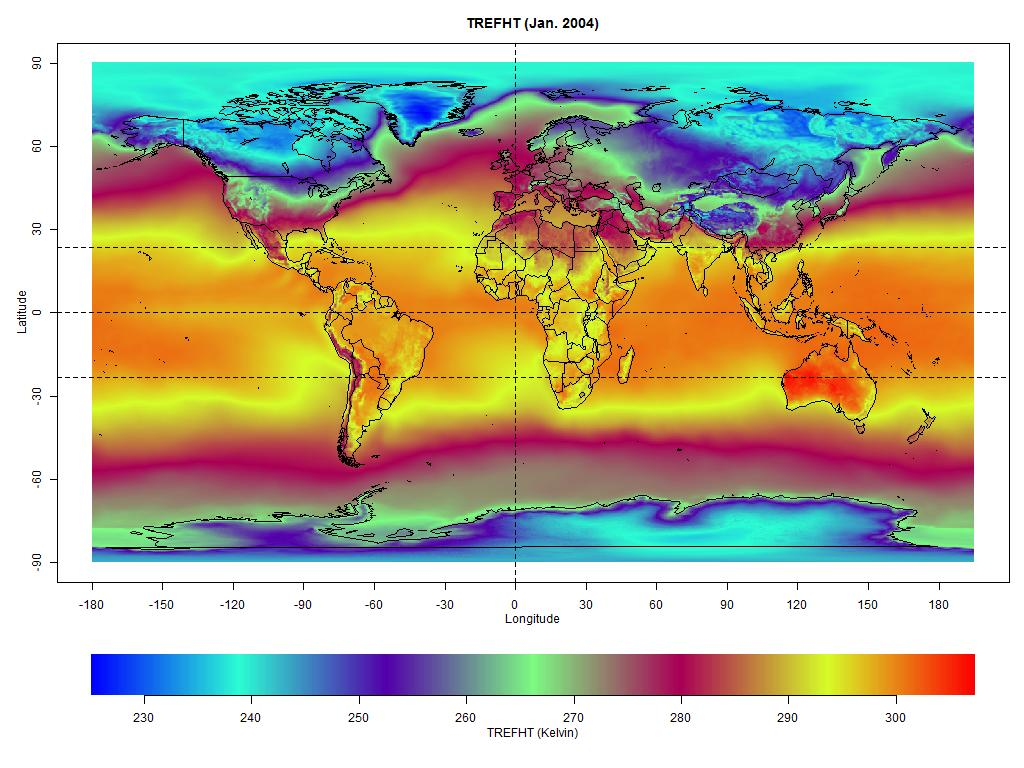
\includegraphics[width=6.0in]{pbdDEMO-include/pics/trefht.jpg}
  \caption[Monthly averaged temperature]{Monthly averaged temperature at reference height (TREFHT) in
           Kelvin (K) for the January 2004. Water freezes at 273.15K and
           boils at 373.15K.}
  \label{fig:trefht}
\end{figure}

A user with \pkg{pbdDEMO} installed can load the \code{TREFHT} dataset in 
the usual way, namely \code{data(TREFHT)} after loading the \pkg{pbdDEMO} 
package.  Here, \code{TREFHT} is a list consisting of several elements. First, 
\code{TREFHT\$def} contains all definitions regarding to this variable in
class \code{ncvar4}\index{Class!\code{ncvar4}} including locations, dimensions, 
units, variable size, data storage, missing values, etc. 

Next, \code{TREFHT\$def\$size} gives the data dimensions which are
$(lon, lat, time) = (1152, 768, 1)$. Since this data is monthly averaged
of Jan. 2004, it is stored as an one-time step output which is
an averaged slice among 20 years.

Finally, \code{TREFHT\$data} contains the values of each
location and is a matrix with dimension $1152\times 768$. Note that the column 
(lon) is in x-axis direction and the row (lat) is in y-axis direction.


\emph{Example: Temperature at reference height (TREFHT).}

In an \proglang{R} session (interactive mode), run the demo by executing
\begin{Code}[title=R Code]
demo(trefht, 'pbdDEMO', ask = F, echo = F)
\end{Code}
This will show a plot as the Figure~\ref{fig:trefht} providing a
visualization about this variable and how temperatures are vary
across locations, particularly decreasing in latitudes. Moreover, the
South hemisphere is hoter than the North hemisphere since the seasonal
effect.



\section{Parallel Write and Read}

\emph{Example: Dump a ddmatrix to a NetCDF4 file and load them from disk.}

The demo command is
\begin{Command}
### At the shell prompt, run the demo with 4 processors by
### (Use Rscript.exe for windows system)
mpiexec -np 4 Rscript -e "demo(nc4_dmat,'pbdDEMO',ask=F,echo=F)"
\end{Command}

Main part of the demo is given in the next:
\begin{lstlisting}[language=rr,title=nc4\_dmat]
### divide data into ddmatrix
x <- TREFHT$data
dx <- as.ddmatrix(x)

# define dimension and variable
lon <- ncdim_def("lon", "degree_east", vals = TREFHT$def$dim[[1]]$vals)
lat <- ncdim_def("lat", "degree_north", vals = TREFHT$def$dim[[2]]$vals)
var.def <- ncvar_def("TREFHT", "K", list(lon = lon, lat = lat), NULL)

### parallel write
file.name <- "nc4_dmat.nc"
nc <- nc_create_par(file.name, var.def)
ncvar_put_dmat(nc, "TREFHT", dx)
nc_close(nc)
if(comm.rank() == 0){
  ncdump(file.name)
}

### parallel read (everyone owns a portion)
nc <- nc_open_par(file.name)
if(comm.rank() == 0){
  print(nc)
}
new.dx <- ncvar_get_dmat(nc, "TREFHT", bldim = bldim(dx), ICTXT = ctxt(dx))
nc_close(nc)
\end{lstlisting}

Line 2 and 3 convert \code{TREFHT\$data} into a \code{ddmatrix} distributed
across 4 processors. Line 6 and 7 define the dimensions
\code{lon} and \code{lat} for longitudes and latitudes, and line 8
defines \code{var.def} as the dumping variable for ``TREFHT'' according
to the dimensions.
 Line 12, 13, and 14 create a parallel NetCDF4 file
\code{nc4_dmat.nc},
write the data into the variable on the disk, and close the file.
Line 20, 24, and 25 open the file again and read the data from the
variable from the data and convert them to a
\code{ddmatrix}.\index{Class!\code{ddmatrix}}

Note that \code{ncvar_put_dmat()} and \code{ncvar_get_dmat()} are implemented
for 2D variables only. Please use \pkg{pbdNCDF4}/\pkg{ncdf4} primitive functions
\code{ncvar_put()} and \code{ncvar_get()} via arguments \code{start}
and \code{count} for more complicated cases. For example, we may write
the \code{TREFHT} into a slice of a hypercube according to it's time step
(Jan. 2004).


\section{Exercises}
\label{sec:pbdNCDF4_exercise}

\begin{enumerate}[label=\thechapter-\arabic*]
\item
The demo code \code{demo/nc4_serial.r} of \pkg{pbdDEMO} has a serial version
of writing and reading \code{TREHFT} as using \pkg{ncdf4} on a single
NetCDF4 file \code{nc4_serial.nc}. It is in the sense of single processor
programming and has low cost if file is not too big.
It is tedious but possible for multiple processors to write
a single file with carefully manual barrier and synchronization.
Modify \code{demo/nc4_serial.r} for writing with multiple processors.

\item
It is also possible to read whole chunk of data from a single processor
and distribute data later manually. Modify the demo code
\code{demo/nc4_parallel.r} to accomplish this goal and make performance
comparisons.

\item
Implement functions or add arguments to \code{ncvar_put_dmat()} and
\code{ncvar_get_dmat()} to enable writing and reading high dimension data,
for example, $(lon, lat, time)$ is 2D in time (3D cube) or
$(lon, lat, lev, time)$ is 3D in time (4D hypercube).
Dump \code{TREFHT} to a slice of 3D cube and load them back to a
\code{ddmatrix}.

\item
In the Sections~\ref{sec:lb_ub} and ~\ref{sec:gbd_dmat}, we introduce
simple matrix distributed formats \code{gbdr} and \code{gbdc} similar to
the BLACS~\index{Library!BLACS} contexts \code{ICTXT} 2 and 1 with very large block size.
The demo code
\code{demo/nc4_gbdc.r} implements similar functionality as for
\code{ddmatrix}, but for \code{gbdc} format only. Modify the demo code for
\code{gbdr} format.
{\color{blue}Hint: See the Exercise~\ref{ex:nc4_gbdr}.
}

\end{enumerate}

